\begin{problem}
{\textbf{\textsc{Liquid Lenses}}} Một giếng tròn lớn, với bán kính 1 mét và chiều sâu lớn hơn nhiều so với bán kính ($d \gg r$), được lấp đầy bằng kim loại lỏng phản xạ ánh sáng. Giếng và chất lỏng bên trong nó sau đó được quay xung quanh trục trung tâm với tốc độ góc $\omega = 5\;\mathrm{rad/s}$, làm cho mép bề mặt chất lỏng dâng lên và chạm vào miệng giếng. Được đặt trực tiếp phía trên giếng là một đèn hình tròn với bán kính $1\;\mathrm{m}$, phát ra photon theo chiều dọc xuống dưới với một tỷ lệ và mật độ đồng đều. Nếu tỷ lệ mà các photon rời khỏi đèn là $r$, thì tỷ lệ mà các photon va chạm với kim loại lỏng có thể được biểu diễn dưới dạng $nr$, với $n$ là một hằng số không có đơn vị. Giá trị của $n$ là bao nhiêu?
% \FloatBarrier 
% \begin{figure}[!htbp]
%      \centering
%     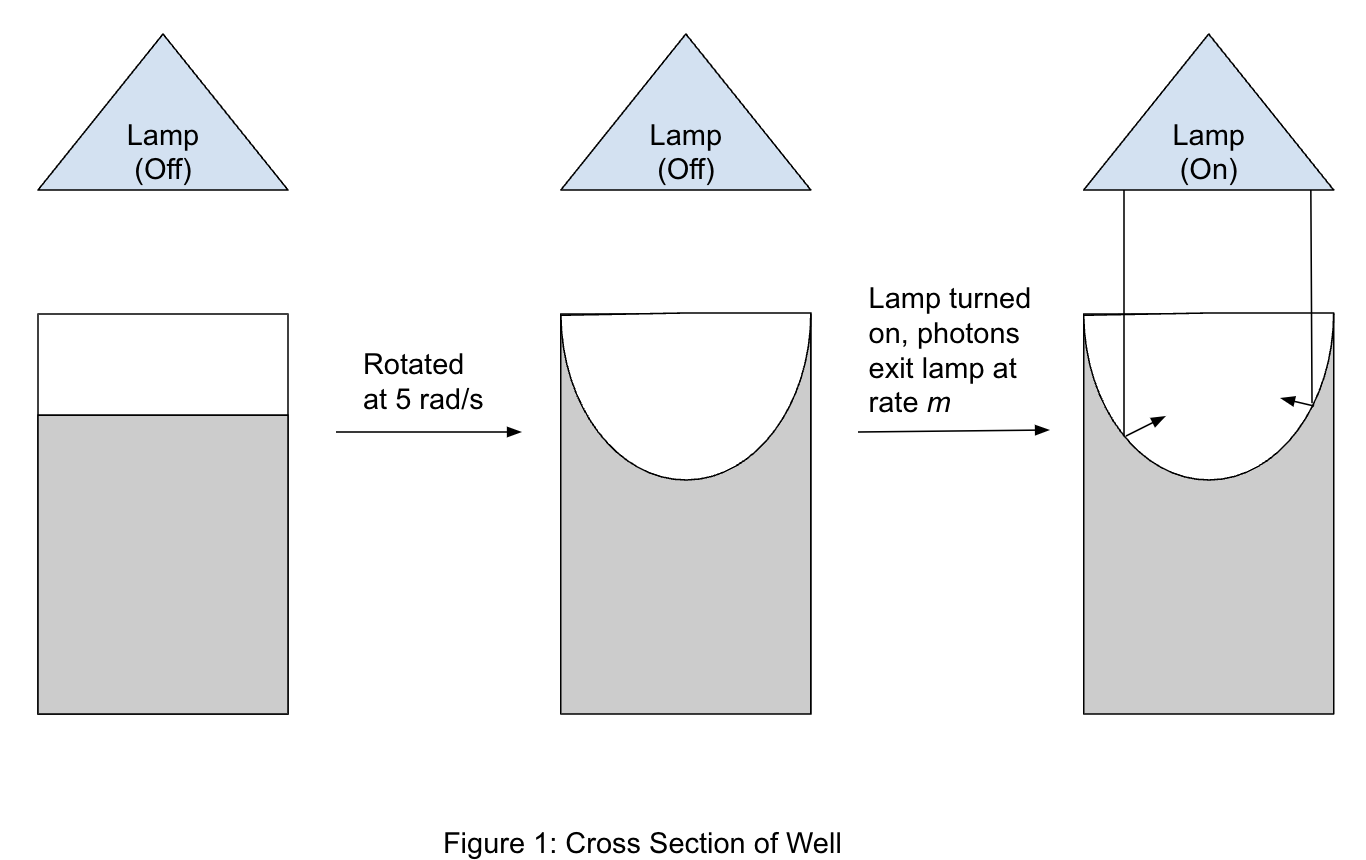
\includegraphics[scale=0.42]{problems/figures/wellDiagram.png}
%  \end{figure}
% \FloatBarrier

\end{problem}